\documentclass[a4paper,oneside]{article}

\usepackage[T1]{fontenc}
\usepackage[utf8]{inputenc}
\usepackage[english]{babel}

\usepackage[margin=2.54cm]{geometry}

\usepackage{amsmath}
\usepackage{amssymb}
\usepackage{siunitx}
\usepackage{hyperref}
\usepackage{color}
\usepackage{graphicx}
\usepackage{subcaption}
\usepackage[section]{placeins}
\usepackage[backend=biber,style=ieee]{biblatex}

\usepackage{customcmds}
\usepackage{codecmds}

\addbibresource{lab3.bib}

\DeclareMathOperator{\clip}{clip}

\author{Riccardo Zanol}
\title{Laboratory 3}

\begin{document}
\matlabcodeconfig
\maketitle
\section*{Experiment 1}
\stepcounter{section}
The purpose of first part of this homework is to implement two
demosaicing algorithms and test them, together with the one
implemented in Matlab, on the eight images \inlinecode{kodimXX.png}
to compare their performances, visually and using the mean squared
error in the CIELAB color space.

Each one of the test images is downsampled by the provided function
\inlinecode{create_bayer} according to the GRBG Bayer mask (see
Fig.~\ref{fig:bayer_grbg}), in order to simulate the kind of data that
would be acquired by a single-sensor imaging system,
\begin{figure}[htbp]
  \centering
  \begin{subfigure}{0.5\textwidth}
    \centering
    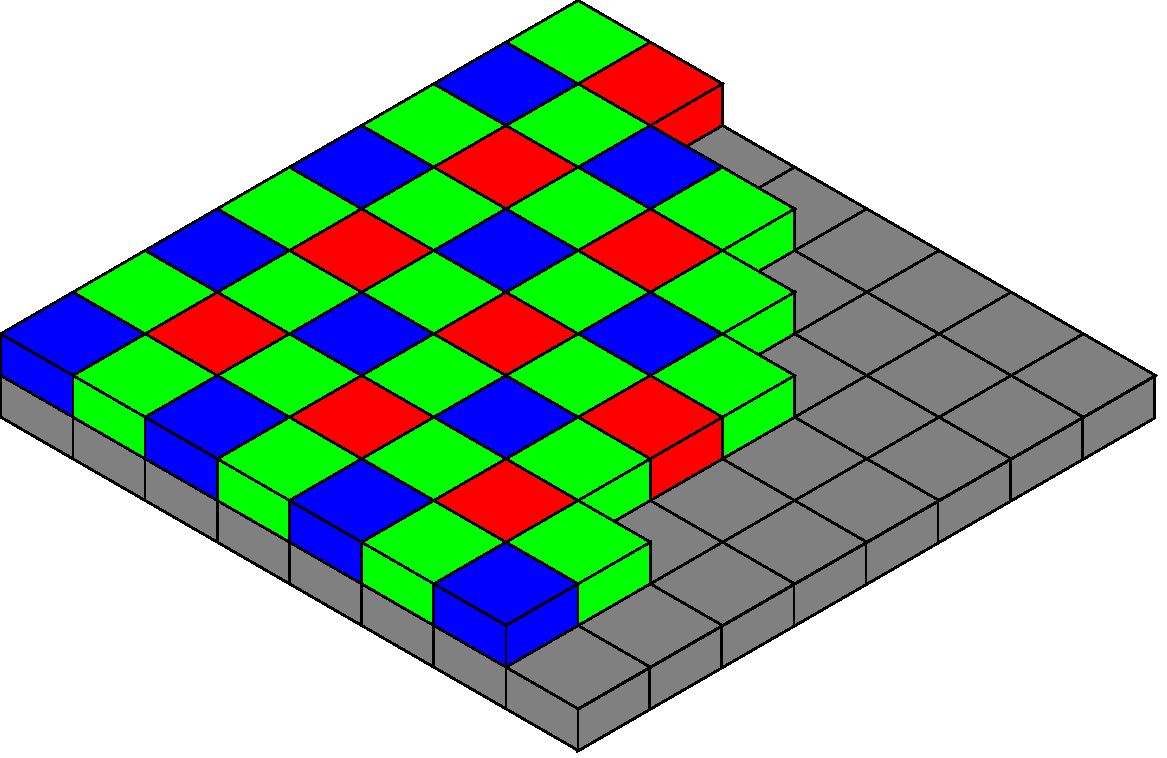
\includegraphics[width=0.66\textwidth]{include_imgs/bayer_grbg}
    \caption{GRBG}
    \label{fig:bayer_grbg}
  \end{subfigure}%
  \begin{subfigure}{0.5\textwidth}
    \centering
    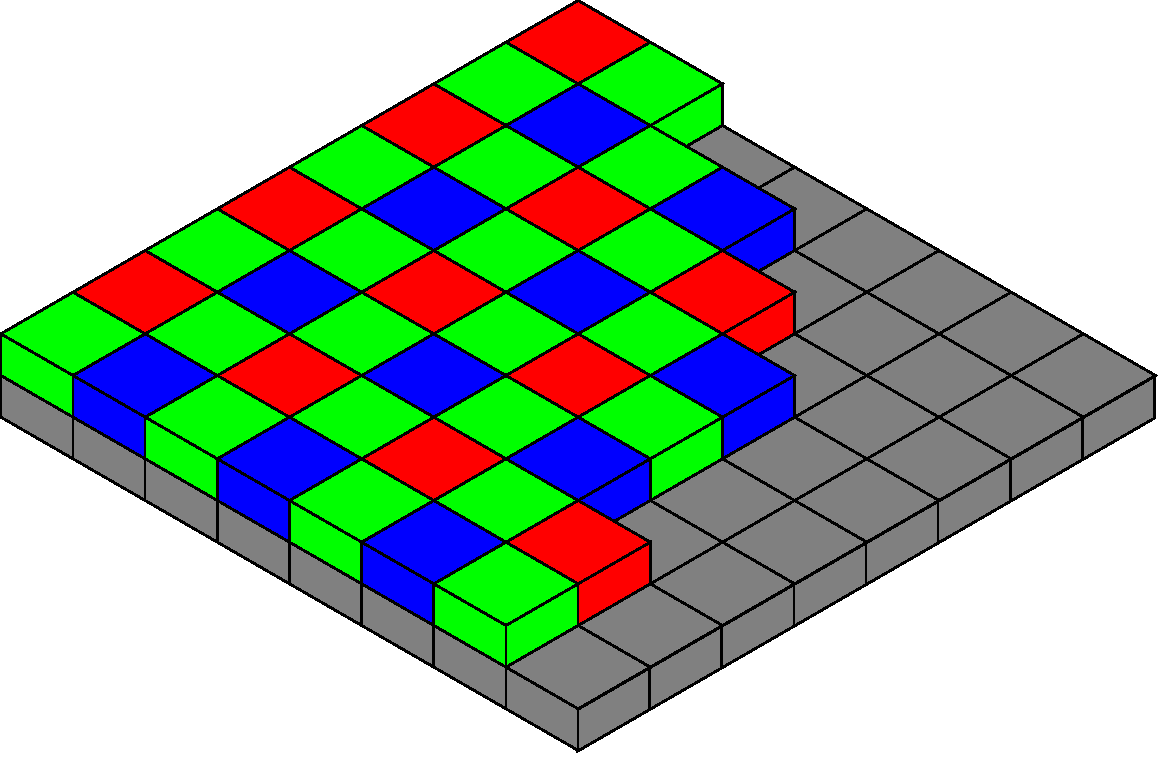
\includegraphics[width=0.66\textwidth]{include_imgs/bayer_rggb}
    \caption{RGGB}
    \label{fig:bayer_rggb}
  \end{subfigure}
  \caption{The two Bayer CFA patterns used in this homework}
\end{figure}
and is then demosaiced using three of the algorithms described in
\cite{demosaic_alg}: the linear interpolation, the gradient-corrected
linear interpolation and a combination of the pattern recognition
interpolation and the smooth hue transition interpolation.

\subsection{Linear interpolation}
\label{sec:linear}
The linear interpolation algorithm is the simplest of the three, it
just sets the missing color components of each pixel to their means in
a 3~by~3 window around the pixel.
%
As an example, in Fig.~\ref{fig:bayer_neigh}, the color of the central
pixel is set to
\begin{align*}
  R_5 &= R_5 \\
  G_5 &= \frac{1}{4}\left( G_2 + G_4 + G_6 + G_8 \right) \\
  B_5 &= \frac{1}{4}\left( B_1 + B_3 + B_7 + B_9 \right) .
\end{align*}
When the algorithm computes the means of the red and blue components
around a green pixel, e.g.~$R_6$~and~$B_6$ in
Fig.~\ref{fig:bayer_neigh}, it takes into account only the two pixels
of the corresponding color that are present in the 3~by~3 window so
\begin{equation*}
  B_6 = \frac{1}{2} \left( B_3 + B_9 \right)
\end{equation*}
and $R_6$ is the mean between $R_5$ and the value at the right of
pixel~6.
%
The same thing also occurs near the picture borders, where there are
only three or two pixels to interpolate the green values and just two
or one pixel to interpolate the other colors.
\begin{figure}[htbp]
  \centering
  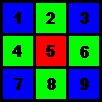
\includegraphics[width=0.20\textwidth]{include_imgs/bayer_neigh}
  \caption{Neighborhood of a red pixel in a Bayer pattern}
  \label{fig:bayer_neigh}
\end{figure}

This algorithm is implemented by the function
\inlinecode{demosaic_linear} and the output images are saved as
\inlinecode{demosaic_kodimXX.png}.

\subsection{Gradient-corrected linear interpolation}
The gradient-corrected linear interpolation is a more complex
algorithm, described in detail in \cite{demosaic_gradient}, that
exploits the correlation between the color components to improve the
quality of the demosaiced image.
%
The mean values of the neighbors, $\hat{r}_{lin}$, $\hat{g}_{lin}$ and
$\hat{b}_{lin}$ computed like in the previous algorithm, are corrected
using the gradient of the color that was measured at that location:
\begin{align*}
  \hat{g}(i,j) &= \hat{g}_{lin}(i,j) + \alpha \Delta_R(i,j) & & \text{red pixel location} \\
  \hat{g}(i,j) &= \hat{g}_{lin}(i,j) + \alpha \Delta_B(i,j) & & \text{blue pixel location} \\
  %
  \hat{r}(i,j) &= \hat{r}_{lin}(i,j) + \beta \Delta_G(i,j) & & \text{green pixel location} \\
  \hat{r}(i,j) &= \hat{r}_{lin}(i,j) + \beta \Delta_B(i,j) & & \text{blue pixel location} \\
  %
  \hat{b}(i,j) &= \hat{b}_{lin}(i,j) + \gamma \Delta_G(i,j) & & \text{green pixel location} \\
  \hat{b}(i,j) &= \hat{b}_{lin}(i,j) + \gamma \Delta_R(i,j) & & \text{red pixel location} \\
\end{align*}
where the gradients are computed on a 5~by~5 window around the pixel
at position $(i,j)$ using a mask that depends on the location and on
the color component that is being interpolated. As an example, when
the green value is interpolated at the location of a red pixel, the
gradient is computed as:
\begin{equation*}
  \Delta_R(i,j) \triangleq r(i,j) - \frac{1}{4} \sum_{(m,n)} r(i+m,j+n)
  \qquad (m,n) \in \{(0,-2), (0,2), (-2,0), (2,0)\} .
\end{equation*}
The gradient-correction gains are chosen in order to minimize the mean
squared error given the statistics of an image set (which contains the
test images used in this homework) and they are approximated to
multiples of small powers of $1/2$: $\alpha = 1/2$, $\beta = 5/8$ and
$\gamma = 3/4$. In \cite{demosaic_gradient} the eight possible masks
for the computation of the gradient are scaled by the
gradient-correction gains and substituted in the six equations above
to obtain eight linear FIR filters to apply to the image.

This algorithm is the one implemented by the built-in Matlab function
\inlinecode{demosaic} and the output images are saved as
\inlinecode{matlab_demosaic_kodimXX.png}.

\subsection{Pattern recognition and smooth hue transition interpolation}
Another demosaicing algorithm described briefly in \cite{demosaic_alg}
and in more detail in \cite{demosaic_army} is the pattern recognition
interpolation, which classifies the pixels into edges, corners and
stripes according to their neighborhood and applies different
interpolation rules for each kind of point.
%
It considers the four neighbors of each missing green pixel and
computes their mean, then labels each neighbor as either ``low'', when
its value is smaller than the mean, or ``high'' otherwise.
%
These labels are used to classify the missing pixel in one of the
categories mentioned above:
\begin{itemize}
\item if three neighbors share the same label the pixel is part of an
  edge (see Fig.s \ref{fig:lowedge} and \ref{fig:highedge}),
\item if two adjacent neighbors share the same label the pixel is part
  of a corner (see Fig. \ref{fig:corner}),
\item
  if two opposite neighbors share the same label the pixel is part of
  a stripe (see Fig. \ref{fig:stripe}).
\item The only missing case, four neighbors with the same intensity, is
  handled like an edge by the code because, as will be seen in the
  next paragraph, this will give the interpolated pixel the median
  value of its neighbors (and so their same value).
\end{itemize}
\begin{figure}[htbp]
  \centering
  \begin{subfigure}{0.2\textwidth}
    \centering
    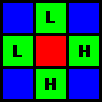
\includegraphics[width=0.8\textwidth]{include_imgs/pri_corner}
    \caption{Corner}
    \label{fig:corner}
  \end{subfigure}%
  \begin{subfigure}{0.2\textwidth}
    \centering
    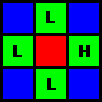
\includegraphics[width=0.8\textwidth]{include_imgs/pri_lowedge}
    \caption{Low edge}
    \label{fig:lowedge}
  \end{subfigure}%
  \begin{subfigure}{0.2\textwidth}
    \centering
    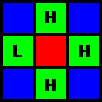
\includegraphics[width=0.8\textwidth]{include_imgs/pri_highedge}
    \caption{High edge}
    \label{fig:highedge}
  \end{subfigure}%
  \begin{subfigure}{0.2\textwidth}
    \centering
    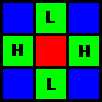
\includegraphics[width=0.8\textwidth]{include_imgs/pri_stripe}
    \caption{Stripe}
    \label{fig:stripe}
  \end{subfigure}
  \caption{Example of classification done by the pattern recognition
    interpolation algorithm}
\end{figure}

After the pixels have been classified, the pattern recognition
algorithm sets their value according to their class:
\begin{itemize}
\item Edge points of both kinds are given the median value of their
  neighbors,
  \item Corner points are given the value $G = \clip_C^B(2M-S)$ where
    $S$ is the mean value of the pixels labeled ``X'' in
    Fig. \ref{fig:mask_corner},
    \item Stripe points are given the value $G = \clip_C^B(2M-S)$ where
    $S$ is the mean value of the pixels labeled ``X'' in
    Fig. \ref{fig:mask_stripe}.
\end{itemize}
In both the stripe and the corner cases above $M$ is the median of the
four closest neighbors, $B$ and $C$ are the values of the second and
the third neighbors taken in descending order ($A \geq B \geq C \geq
D$) and the $\clip$ function is defined as:
\begin{equation*}
  \clip_C^B(x) = \begin{cases}
    B \qquad & x > B \\
    x \qquad & C \leq x \leq B \\
    C \qquad & x < C
    \end{cases} .
\end{equation*}
\begin{figure}[htbp]
  \centering
  \begin{subfigure}{0.33\textwidth}
    \centering
    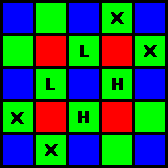
\includegraphics[width=0.9\textwidth]{include_imgs/pri_corner_mask}
    \caption{Corner}
    \label{fig:mask_corner}
  \end{subfigure}%
  \begin{subfigure}{0.33\textwidth}
    \centering
    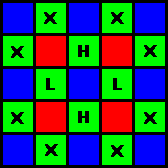
\includegraphics[width=0.9\textwidth]{include_imgs/pri_stripe_mask}
    \caption{Stripe}
    \label{fig:mask_stripe}
  \end{subfigure}
  \caption{Masks used in the computation of the interpolated value}
\end{figure}

There is no mention on \cite{demosaic_alg, demosaic_army} on what the
algorithm should do near the picture border, when there are not enough
neighbors, however this is just a small two-pixel border so it should
not affect the performances so much.
%
If the four closest neighbors are not available the pixel cannot be
classified so the code uses the same linear interpolation algorithm of
section \ref{sec:linear}.
%
When, instead, the pixel can be classified but the ``X'' pixels of
Fig.s \ref{fig:mask_corner} and \ref{fig:mask_stripe} are not all
available, the mean $S$ is computed using only the ones that fall
inside the picture.

This algorithm is designed to work only on the green component so, in
order to perform a complete demosaicing of an image, another algorithm
must be used to interpolate the other colors. A suggestion given by
\cite{demosaic_alg, demosaic_army} is to use the smooth hue transition
interpolation algorithm, which assumes that the hue changes smoothly
across an object's surface and so it uses the ratio between the blue
or red components and the green component instead of their absolute
values.
%
The red-green and blue-green ratios are linearly interpolated, with
the same rules of section \ref{sec:linear}. As an example, the blue
component is interpolated in Fig.~\ref{fig:bayer_neigh} using
\begin{align*}
  B_2 &= G_2 \frac{1}{2} \left( \frac{B_1}{G_1} + \frac{B_3}{G_3} \right) \\
  B_4 &= G_4 \frac{1}{2} \left( \frac{B_1}{G_1} + \frac{B_7}{G_7} \right) \\
  B_5 &= G_5 \frac{1}{4} \left( \frac{B_1}{G_1} + \frac{B_3}{G_3} +
  \frac{B_7}{G_7} +\frac{B_9}{G_9}\right) .
\end{align*}
This method fails if some green values are zero, but the
transformation
\begin{equation*}
  \frac{B}{G} \rightarrow \frac{B + \beta}{ G + \beta} \qquad \beta > 0
\end{equation*}
can be used to avoid this issue.
%
With this transformation the previous equations become
\begin{align*}
  B_2 &= -\beta + \left(G_2 +\beta \right) \frac{1}{2} \left(
  \frac{B_1 + \beta}{G_1 + \beta} + \frac{B_3 + \beta}{G_3 + \beta} \right) \\
  B_4 &= -\beta + \left( G_4 + \beta \right) \frac{1}{2} \left(
  \frac{B_1 + \beta}{G_1 + \beta} + \frac{B_7 + \beta}{G_7 + \beta} \right) \\
  B_5 &= -\beta + \left( G_5 +\beta \right) \frac{1}{4} \left(
  \frac{B_1 + \beta}{G_1 + \beta} + \frac{B_3 + \beta}{G_3 + \beta} +
  \frac{B_7 + \beta}{G_7 + \beta} +\frac{B_9 + \beta}{G_9 + \beta}\right) .
\end{align*}
The value of $\beta$ that is suggested by \cite{demosaic_army} is
$\beta = 128$.

The pattern recognition interpolation and the smooth hue transition
interpolation algorithms are implemented, respectively, in the
functions \inlinecode{pattern_interp} and \inlinecode{smooth_hue} and
used together by the function \inlinecode{demosaic_pattern_hue} to
perform the demosaicing. The output images are saved as
\inlinecode{prsh_demosaic_kodimXX.png}.

\subsection{Comparison}
After the images have been demosaiced by each one of the three
algorithms, they are converted from the sRGB to the CIELAB color space
and the MSE between the output and the original images is
computed. The MSE between $A$ and $B$ is computed by taking the
euclidean distance between the colors of each corresponding pixel and
averaging over the image:
\begin{align*}
  d(i,j) &= \sqrt{\sum_{k=1}^3 \left(A(i,j,k) - B(i,j,k)\right)^2 } \\
  \text{MSE} &= \frac{1}{WH}\sum_{i=0}^H\sum_{j=0}^Wd(i,j)
\end{align*}
where $A(i,j,1) = L_A(i,j)$, $A(i,j,2) = a_A(i,j)$ and $A(i,j,3) =
b_A(i,j)$ are the three coordinates in the CIELAB space of the pixel
$(i,j)$ of image $A$.
%
The computed values of the MSE are shown in Tab.~\ref{tab:mse} where
it can be seen that the gradient-corrected linear interpolation is,
with respect to the MSE, always the best algorithm followed by the
pattern recognition and smooth hue transition interpolation
algorithms, while the linear interpolation always gives the highest
MSE.
\begin{table}[h]
  \centering
  \begin{tabular}{IRRR}
    \multicolumn{1}{c}{Image} &
    \multicolumn{1}{c}{Linear} &
    \multicolumn{1}{c}{Gradient-corrected} &
    \multicolumn{1}{c}{PRI and SHTI} \\
    \hline
    kodim01.png & 5.053 & 2.909 & 3.434 \\
    kodim05.png & 4.637 & 2.407 & 3.242 \\
    kodim13.png & 6.275 & 3.707 & 4.850 \\
    kodim19.png & 3.333 & 1.974 & 2.236 \\
  \end{tabular}
  \caption{Mean squared error of the three tested demosaicing
    algorithms }
  \label{tab:mse}
\end{table}

A visual comparison of the demosaiced images with the original,
however, shows that the MSE is not always a good indicator of the
performances of the algorithms (see Fig.s \ref{fig:wall} and
\ref{fig:door}).
%
The linear interpolation algorithm is the worst performing one, since
it creates a lot of artifacts in the output images, especially along
the edges. It also slightly blurs the image because it interpolates
the pixels on the edges using samples from both sides.
%
The gradient-corrected interpolation works better and the resulting
image is less blurred, but it still leaves very noticeable zippering
and false color artifacts.
%
The pattern recognition algorithm is designed specifically to avoid
interpolating across an edge so, as expected, it reduces a lot these
two kind of artifacts, even if it not able to completely eliminate
them.
%
It also alters some small details, like the door knob in
Fig. \ref{fig:door} that becomes a square, and this may be the cause
for its higher MSE value than the gradient-corrected algorithm, even
if the resulting images look closer to the original ones.
%
Another reason for the mismatch between the MSE comparison and the
visual comparison may be that these particular images were part of the
set used to optimize the gradient-correction gain for the minimum MSE,
so if new images were used they would maybe yield worse MSE values.
\begin{figure}[htbp]
  \centering
  \begin{subfigure}{0.4\textwidth}
    \centering
    \includegraphics[width=0.95\textwidth]{include_imgs/generated/kodim19_wall}
    \caption{Original}
  \end{subfigure}%
  \begin{subfigure}{0.4\textwidth}
    \centering
    \includegraphics[width=0.95\textwidth]{include_imgs/generated/demosaic_kodim19_wall}
    \caption{Linear interpolation}
  \end{subfigure}
  \begin{subfigure}{0.4\textwidth}
    \centering
    \includegraphics[width=0.95\textwidth]{include_imgs/generated/matlab_demosaic_kodim19_wall}
    \caption{Gradient-corrected linear interpolation}
  \end{subfigure}%
  \begin{subfigure}{0.4\textwidth}
    \centering
    \includegraphics[width=0.95\textwidth]{include_imgs/generated/prsh_demosaic_kodim19_wall}
    \caption{PR and SHT interpolation}
  \end{subfigure}
  \caption{Comparison of some artifacts in \inlinecode{kodim_19.png}
    introduced by the demosaicing}
  \label{fig:wall}
\end{figure}
Another disadvantage of the demosaicing performed with the pattern
recognition and the smooth hue transition interpolation is that they
are non-linear (unlike the other two approaches) and require more
computational resources.
\begin{figure}[htbp]
  \centering
  \begin{subfigure}{0.4\textwidth}
    \centering
    \includegraphics[width=0.95\textwidth]{include_imgs/generated/kodim01_door}
    \caption{Original}
  \end{subfigure}%
  \begin{subfigure}{0.4\textwidth}
    \centering
    \includegraphics[width=0.95\textwidth]{include_imgs/generated/demosaic_kodim01_door}
    \caption{Linear interpolation}
  \end{subfigure}
  \begin{subfigure}{0.4\textwidth}
    \centering
    \includegraphics[width=0.95\textwidth]{include_imgs/generated/matlab_demosaic_kodim01_door}
    \caption{Gradient-corrected linear interpolation}
  \end{subfigure}%
  \begin{subfigure}{0.4\textwidth}
    \centering
    \includegraphics[width=0.95\textwidth]{include_imgs/generated/prsh_demosaic_kodim01_door}
    \caption{PR and SHT interpolation}
  \end{subfigure}
  \caption{Comparison of some artifacts in \inlinecode{kodim_01.png}
    introduced by the demosaicing}
  \label{fig:door}
\end{figure}

\section*{Experiment 2}
The matlab script \inlinecode{ex2.m} applies the same two demosaicing
algorithms to some images acquired from a reflex camera. This time,
since it starts from the raw sensor data, it has to perform some
additional steps to get an output that can be compared to the JPEG
files produced by the camera. The script reads the DNG files using the
provided function \inlinecode{read_dng}, which also performs the
linearization and white balancing of the image using the meta-data
stored with it, then it applies the same two demosaicing algorithms
of experiment 1.

The raw data of the image is stored according to a ``RGGB'' Bayer
pattern so the script adds one column of zeros at the beginning and at
the end of the image, in this way it shifts the pattern horizontally
by one pixel and it becomes the ``GRBG'' pattern that the function
\inlinecode{demosaic_linear} expects. The extra columns do not affect
the demosaicing results because this function skips a two pixel wide
border around the image.  The built-in \inlinecode{demosaic} function
could work directly on the ``RGGB'' pattern, but since the two columns
must be added anyway the script uses it in the same way of experiment
1. This function also requires the input pixels to be of type
\inlinecode{uint8} so the image is converted before the demosaicing.

After the demosaicing step, the image is post-processed with the
provided \inlinecode{post_process} function that normalizes the image
intensity and applies a gamma correction.

Comparing the results with the JPEG files produced by the camera it
can be seen that the steps that are skipped in the raw image processing
affect the color, in particular the \inlinecode{post_process} function
does not convert the image from the color space of the camera to
sRGB. As can be seen in Fig.~\ref{fig:chart} the result images appear
to have a much lower contrast than the camera JPEG file.
\begin{figure}[htbp]
  \centering
  \begin{subfigure}{.33\textwidth}
  \centering
  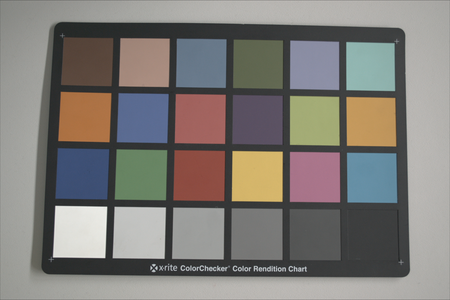
\includegraphics[width=.95\linewidth]{demosaic_macbeth_color_small}
  \caption{\inlinecode{demosaic_linear}}
\end{subfigure}%
\begin{subfigure}{.33\textwidth}
  \centering
  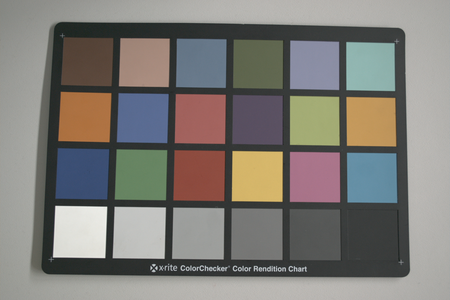
\includegraphics[width=.95\linewidth]{matlab_demosaic_macbeth_color_small}
  \caption{\inlinecode{demosaic}}
\end{subfigure}%
  \begin{subfigure}{.33\textwidth}
  \centering
  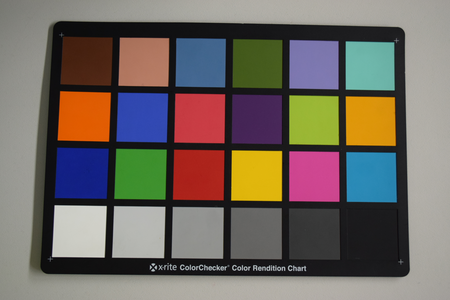
\includegraphics[width=.95\linewidth]{camera_macbeth_color_small}
  \caption{JPEG from the camera}
\end{subfigure}
\caption{Comparison of the color chart}
\label{fig:chart}
\end{figure}
The demosaicing performed by the matlab script also leaves a lot of
artifacts, especially in the dark areas as can be seen from
Fig.~\ref{fig:dark_artifacts}. In this case the linear interpolation
algorithm appears to produce slightly better images than the gradient
corrected one, but they are both very noisy compared to the camera's
processed images.
\begin{figure}[htbp]
  \centering
  \begin{subfigure}{.33\textwidth}
  \centering
  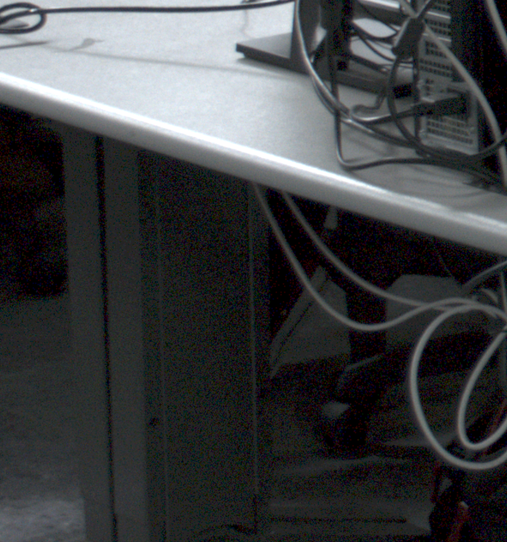
\includegraphics[width=.95\linewidth]{demosaic_students2_detail}
  \caption{\inlinecode{demosaic_linear}}
\end{subfigure}%
\begin{subfigure}{.33\textwidth}
  \centering
  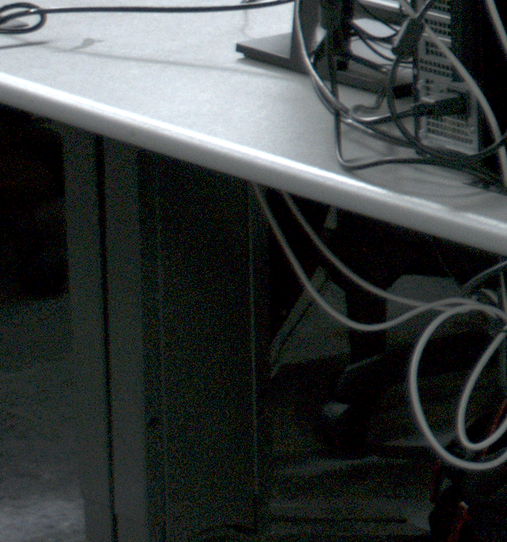
\includegraphics[width=.95\linewidth]{matlab_demosaic_students2_detail}
  \caption{\inlinecode{demosaic}}
\end{subfigure}%
  \begin{subfigure}{.33\textwidth}
  \centering
  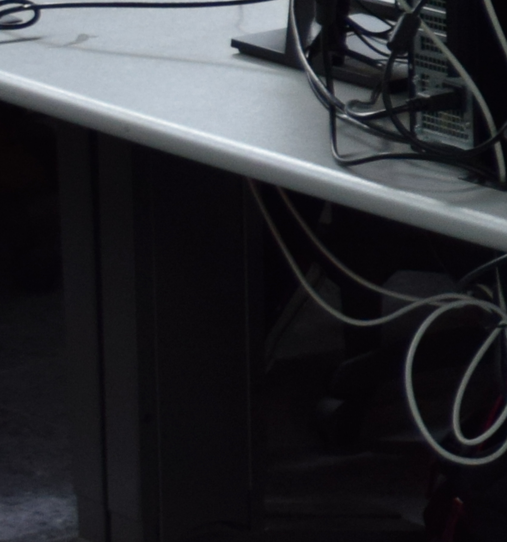
\includegraphics[width=.95\linewidth]{camera_students2_detail}
  \caption{JPEG from the camera}
\end{subfigure}
\caption{Comparison of a detail from \inlinecode{students2.dng}}
\label{fig:dark_artifacts}
\end{figure}

\printbibliography
\end{document}
